% ======================================================================
%  Chapter 3 — Normal Modes and the Electromagnetic Inner Product
% ======================================================================

\section{Why the inner product matters}
\label{sec:ch3-why-ip}

In quantum mechanics, the Hilbert-space inner product
$\langle\psi|\phi\rangle=\int\psi^*\phi\,\dd^3r$ is so natural that it
is rarely questioned.  The Hamiltonian is self-adjoint under this inner
product, eigenvalues are real, and eigenstates are orthogonal---all
with the standard $L^2$ norm.

The Maxwell eigenvalue equation
\begin{equation}\label{eq:ch3-evp-recap}
  \Maxop\,\emfield = \omega\,\Mmat\,\emfield
\end{equation}
from \chref{ch:maxwell-dynamics} is \emph{not} a standard eigenvalue
problem.  The material matrix $\Mmat$ appears on the right-hand side,
making this a \emph{generalised} eigenproblem.  If we naively define an
``effective Hamiltonian'' $\Hamop=\Mmat^{-1}\Maxop$ and write
$\Hamop\emfield=\omega\emfield$, the operator $\Hamop$ is generally
\emph{not} Hermitian under the standard inner product
$\emfield_1^\dagger\emfield_2$.

This means that the standard $L^2$ inner product is the \emph{wrong}
inner product for electromagnetic normal modes.  Using it leads to
non-orthogonal modes, non-gauge-invariant Berry connections, and
incorrect topological invariants.  The correct inner product is the
\emph{electromagnetic energy inner product}, weighted by the material
matrix $\Mmat$ (or, in dispersive media, by the energy metric
$\Mgmat$) \cite{nittis2020equivalence}.  Establishing this inner product rigorously is the central
task of this chapter.

\section{Self-adjointness of the Maxwell operator}
\label{sec:ch3-self-adjoint}

\subsection{The nondispersive case}
\label{sec:ch3-self-adjoint-nondisp}

Consider first a nondispersive lossless medium, so that $\Mmat(\rvec)$
is Hermitian and frequency-independent.  Define the electromagnetic
inner product over a domain $V$ (which will later be specialised to a
unit cell):
\begin{equation}\label{eq:ch3-em-ip}
  \boxed{%
  \emip{\emfield_1}{\emfield_2}
  \;\equiv\;
  \int_V \emfield_1^\dagger(\rvec)\cdot\Mmat(\rvec)
         \cdot\emfield_2(\rvec)\,\dd^3r\,.}
\end{equation}
Since $\Mmat=\Mmat^\dagger$, this is a sesquilinear form; since $\Mmat$
is positive definite (\secref{sec:ch2-dispersive-energy}), it is
positive definite and hence a genuine inner product.

\begin{theorem}[Self-adjointness of the Maxwell operator]
  \label{thm:ch3-self-adjoint}
  Let $\Mmat(\rvec)$ be Hermitian and positive definite, and let
  $\emfield_1$, $\emfield_2$ be smooth six-component fields satisfying
  appropriate boundary conditions (periodic, or vanishing at infinity).
  Then the Maxwell curl operator $\Maxop$ is self-adjoint with respect
  to the electromagnetic inner product:
  \begin{equation}\label{eq:ch3-self-adj-statement}
    \emip{\emfield_1}{\Mmat^{-1}\Maxop\,\emfield_2}
    = \emip{\Mmat^{-1}\Maxop\,\emfield_1}{\emfield_2}\,.
  \end{equation}
  Equivalently, writing $\Hamop=\Mmat^{-1}\Maxop$:
  \begin{equation}\label{eq:ch3-H-self-adj}
    \emip{\emfield_1}{\Hamop\,\emfield_2}
    = \emip{\Hamop\,\emfield_1}{\emfield_2}\,.
  \end{equation}
\end{theorem}

\begin{proof}
We need to show that
\begin{equation}\label{eq:ch3-proof-target}
  \int_V \emfield_1^\dagger\,\Mmat\,(\Mmat^{-1}\Maxop\,\emfield_2)\,\dd^3r
  = \int_V (\Mmat^{-1}\Maxop\,\emfield_1)^\dagger\,\Mmat\,\emfield_2\,\dd^3r\,.
\end{equation}
The left-hand side simplifies to $\int_V\emfield_1^\dagger\,\Maxop\,\emfield_2\,\dd^3r$.
The right-hand side simplifies to
$\int_V(\Maxop\,\emfield_1)^\dagger\,\Mmat^{-\dagger}\Mmat\,\emfield_2\,\dd^3r
=\int_V(\Maxop\,\emfield_1)^\dagger\,\emfield_2\,\dd^3r$
since $\Mmat^{-\dagger}\Mmat=\mathbf{I}$ for Hermitian $\Mmat$.
So we need to prove
\begin{equation}\label{eq:ch3-maxop-sa}
  \int_V \emfield_1^\dagger\,\Maxop\,\emfield_2\,\dd^3r
  = \int_V (\Maxop\,\emfield_1)^\dagger\,\emfield_2\,\dd^3r\,,
\end{equation}
i.e., $\Maxop$ itself is self-adjoint under the \emph{standard} $L^2$
inner product.

Write $\emfield_i=(\Efield_i,\Hfield_i)^T$.  Then
\begin{equation}
  \emfield_1^\dagger\,\Maxop\,\emfield_2
  = \Efield_1^*\cdot(\ii\nabla\times\Hfield_2)
    + \Hfield_1^*\cdot(-\ii\nabla\times\Efield_2)\,.
\end{equation}
Similarly,
\begin{equation}
  (\Maxop\,\emfield_1)^\dagger\,\emfield_2
  = (-\ii\nabla\times\Hfield_1)^*\cdot\Efield_2
    + (\ii\nabla\times\Efield_1)^*\cdot\Hfield_2
  = \ii(\nabla\times\Hfield_1^*)\cdot\Efield_2
    - \ii(\nabla\times\Efield_1^*)\cdot\Hfield_2\,.
\end{equation}
Taking the difference:
\begin{align}
  &\emfield_1^\dagger\,\Maxop\,\emfield_2
   - (\Maxop\,\emfield_1)^\dagger\,\emfield_2 \notag\\
  &= \ii\bigl[
    \Efield_1^*\cdot(\nabla\times\Hfield_2)
    - (\nabla\times\Hfield_1^*)\cdot\Efield_2
  \bigr]
  -\ii\bigl[
    \Hfield_1^*\cdot(\nabla\times\Efield_2)
    - (\nabla\times\Efield_1^*)\cdot\Hfield_2
  \bigr]. \label{eq:ch3-sa-diff}
\end{align}
Each bracket is a total divergence.  Using the identity
$\mathbf{A}\cdot(\nabla\times\mathbf{B})
-(\nabla\times\mathbf{A})\cdot\mathbf{B}
= -\nabla\cdot(\mathbf{A}\times\mathbf{B})$:
\begin{equation}\label{eq:ch3-sa-divergence}
  \emfield_1^\dagger\,\Maxop\,\emfield_2
  - (\Maxop\,\emfield_1)^\dagger\,\emfield_2
  = -\ii\,\nabla\cdot\bigl(
    \Efield_1^*\times\Hfield_2
    - \Hfield_1^*\times\Efield_2
  \bigr).
\end{equation}
Integrating over $V$ and applying the divergence theorem:
\begin{equation}\label{eq:ch3-boundary-term}
  \int_V\bigl(\emfield_1^\dagger\,\Maxop\,\emfield_2
  - (\Maxop\,\emfield_1)^\dagger\,\emfield_2\bigr)\dd^3r
  = -\ii\oint_{\partial V}\bigl(
    \Efield_1^*\times\Hfield_2
    - \Hfield_1^*\times\Efield_2
  \bigr)\cdot\hat{n}\,\dd A\,.
\end{equation}
The surface integral vanishes when:
\begin{enumerate}[label=(\alph*)]
  \item the fields satisfy \emph{periodic boundary conditions}
    ($\emfield(\rvec+\avec)=\ee^{\ii\kvec\cdot\avec}\emfield(\rvec)$
    for lattice vector $\avec$), since opposite faces of the unit cell
    contribute equal and opposite terms; or
  \item the fields decay sufficiently fast at infinity; or
  \item the domain has perfectly conducting or perfectly magnetic boundaries.
\end{enumerate}
Under any of these conditions,
$\int_V\emfield_1^\dagger\Maxop\emfield_2\,\dd^3r
=\int_V(\Maxop\emfield_1)^\dagger\emfield_2\,\dd^3r$,
establishing \eqref{eq:ch3-maxop-sa} and hence
\eqref{eq:ch3-H-self-adj}.
\end{proof}

\begin{corollary}[Real eigenfrequencies]
  \label{cor:ch3-real-omega}
  Every eigenfrequency $\omega_n$ of the Maxwell normal-mode problem
  $\Hamop\emfield_n=\omega_n\emfield_n$ is real.
\end{corollary}

\begin{proof}
From self-adjointness:
$\omega_n\emip{\emfield_n}{\emfield_n}
=\emip{\emfield_n}{\Hamop\emfield_n}
=\emip{\Hamop\emfield_n}{\emfield_n}
=\omega_n^*\emip{\emfield_n}{\emfield_n}$.
Since $\emip{\emfield_n}{\emfield_n}>0$, we conclude $\omega_n=\omega_n^*$.
\end{proof}

\subsection{Orthogonality of modes}
\label{sec:ch3-orthogonality} \cite{press2026photonic}

\begin{proposition}[Mode orthogonality]
  \label{prop:ch3-orthogonality}
  Eigenmodes at different eigenfrequencies are orthogonal under the
  electromagnetic inner product:
  \begin{equation}\label{eq:ch3-orthogonality}
    \omega_n\neq\omega_m
    \quad\Longrightarrow\quad
    \emip{\emfield_n}{\emfield_m}=0\,.
  \end{equation}
\end{proposition}

\begin{proof}
Self-adjointness gives
$\emip{\emfield_n}{\Hamop\emfield_m}
=\emip{\Hamop\emfield_n}{\emfield_m}$, i.e.,
$\omega_m\emip{\emfield_n}{\emfield_m}
=\omega_n^*\emip{\emfield_n}{\emfield_m}
=\omega_n\emip{\emfield_n}{\emfield_m}$
(using $\omega_n\in\mathbb{R}$).  Hence
$(\omega_m-\omega_n)\emip{\emfield_n}{\emfield_m}=0$; if
$\omega_n\neq\omega_m$, the inner product vanishes.
\end{proof}

We adopt the \emph{energy normalisation convention}:
\begin{equation}\label{eq:ch3-normalisation}
  \emip{\emfield_n}{\emfield_m}
  = \int_V\emfield_n^\dagger\,\Mmat\,\emfield_m\,\dd^3r
  = \delta_{nm}\,.
\end{equation}
The physical meaning of $\emip{\emfield_n}{\emfield_n}=1$ is that the
mode carries unit time-averaged electromagnetic energy per unit cell (in
a periodic medium) or per normalisation volume.

\section{The energy-weighted field}
\label{sec:ch3-energy-weighted}

The electromagnetic inner product \eqref{eq:ch3-em-ip} is perfectly
rigorous \cite{gangaraj2016berry,raghu2008analogs}, but it is sometimes convenient to work with a
\emph{standard}-Hermitian formulation.  This is achieved by a change of
variables that absorbs $\Mmat$ into the field.

Since $\Mmat$ is Hermitian and positive definite, it has a unique
positive-definite Hermitian square root $\Mmat^{1/2}$.  Define the
\emph{energy-weighted field}
\begin{equation}\label{eq:ch3-w-def}
  \boxed{%
  \emfieldw(\rvec) \equiv \Mmat^{1/2}(\rvec)\,\emfield(\rvec)\,.}
\end{equation}
Then the electromagnetic inner product becomes the standard $L^2$ inner
product for $\emfieldw$:
\begin{equation}\label{eq:ch3-w-ip}
  \emip{\emfield_1}{\emfield_2}
  = \int_V\emfield_1^\dagger\Mmat\emfield_2\,\dd^3r
  = \int_V\emfieldw_1^\dagger\,\emfieldw_2\,\dd^3r\,.
\end{equation}
The eigenvalue equation in terms of $\emfieldw$ becomes
\begin{equation}\label{eq:ch3-w-evp}
  \tilde{\Hamop}(\rvec)\,\emfieldw(\rvec)
  = \omega\,\emfieldw(\rvec)\,,
  \qquad
  \tilde{\Hamop}
  = \Mmat^{-1/2}\,\Maxop\,\Mmat^{-1/2}\,,
\end{equation}
and $\tilde{\Hamop}$ is Hermitian under the standard inner product.

\begin{remark}
The energy-weighted formulation is useful for formal proofs and for
connecting to the quantum-mechanical literature, where Berry connections
are always defined with respect to the standard inner product.  However,
the original formulation in terms of $\emfield$ and $\Mmat$ is often
more convenient in practice, because $\emfield=(\Efield,\Hfield)^T$
has direct physical meaning, while $\emfieldw=\Mmat^{1/2}\emfield$ does
not correspond to any simply measurable field.  We will use both
formulations interchangeably and state which inner product is being used
at each stage.
\end{remark}

\section{Extension to dispersive media}
\label{sec:ch3-dispersive}

\subsection{The generalised eigenvalue problem}
\label{sec:ch3-gen-evp}

Real magneto-optical materials are always dispersive: the gyrotropic
parameter $\kappa$ in \eqref{eq:ch2-gyrotropic-mu} depends on
frequency, as do $\varepsilon$, $\mu_\perp$, and all other material
parameters
\cite{wang2007reflection}.  The material matrix is then $\Mmat=\Mmat(\rvec,\omega)$,
and the Maxwell eigenvalue equation
\begin{equation}\label{eq:ch3-gen-evp}
  \Maxop\,\emfield = \omega\,\Mmat(\omega)\,\emfield
\end{equation}
is a \emph{nonlinear} eigenvalue problem in $\omega$: the eigenvalue
appears both explicitly and inside $\Mmat$.  This is qualitatively
different from the Schr\"odinger equation, where the Hamiltonian does
not depend on the energy eigenvalue.

Following Haldane and Raghu, we treat this as a generalised eigenvalue
problem.  For a Bloch mode in a periodic medium, the cell-periodic
eigenproblem takes the form
\begin{equation}\label{eq:ch3-bloch-gen-evp}
  \Maxop(\kvec)\,\mathbf{u}_{n\kvec}(\rvec)
  = \omega_{n\kvec}\,\Mmat(\rvec,\omega_{n\kvec})\,
    \mathbf{u}_{n\kvec}(\rvec)\,,
\end{equation}
where $\Maxop(\kvec)$ is the curl operator with $\nabla$ replaced by
$\nabla+\ii\kvec$ (incorporating the Bloch phase).

\subsection{The energy metric as inner product}
\label{sec:ch3-energy-metric-ip}

The self-adjointness proof of \secref{sec:ch3-self-adjoint-nondisp}
relied on $\Mmat$ being the same for both modes.  In the dispersive
case, two modes $\emfield_n$ and $\emfield_m$ at \emph{different}
frequencies see \emph{different} material matrices
$\Mmat(\omega_n)\neq\Mmat(\omega_m)$, and the standard orthogonality
argument breaks down.

The resolution was provided by the energy metric
$\Mgmat(\omega)=\partial_\omega[\omega\Mmat(\omega)]$ introduced in
\eqref{eq:ch2-energy-metric}.  The key result is:

\begin{theorem}[Orthogonality in dispersive media]
  \label{thm:ch3-dispersive-orth}
  Let $\Mmat(\rvec,\omega)$ be Hermitian for real $\omega$, and let
  $\Mgmat(\rvec,\omega)=\partial_\omega[\omega\Mmat(\rvec,\omega)]$ be
  positive definite at all physical eigenfrequencies.  Then two Bloch
  eigenmodes $\mathbf{u}_{n\kvec}$ and $\mathbf{u}_{m\kvec}$ at the
  same wavevector $\kvec$ but different frequencies satisfy the
  \emph{exact} relation
  \begin{equation}\label{eq:ch3-dispersive-orth}
    \omega_n\int_{\mathrm{cell}}
    \mathbf{u}_{n\kvec}^\dagger\,\Mmat(\omega_n)
    \,\mathbf{u}_{m\kvec}\,\dd^3r
    = \omega_m\int_{\mathrm{cell}}
    \mathbf{u}_{n\kvec}^\dagger\,\Mmat(\omega_m)
    \,\mathbf{u}_{m\kvec}\,\dd^3r\,.
  \end{equation}
  When the two frequencies are close ($\omega_m\to\omega_n$), this
  reduces to $\int\mathbf{u}_n^\dagger\Mgmat(\omega_n)\mathbf{u}_m
  \,\dd^3r=0$.  The group-velocity metric $\Mgmat$ therefore plays
  the role of the orthogonality metric for near-degenerate modes and
  also determines the self-overlap normalization
  $\int\mathbf{u}_n^\dagger\Mgmat(\omega_n)\mathbf{u}_n\,\dd^3r>0$.
\end{theorem}

\begin{figure}[!t]
  \centering
  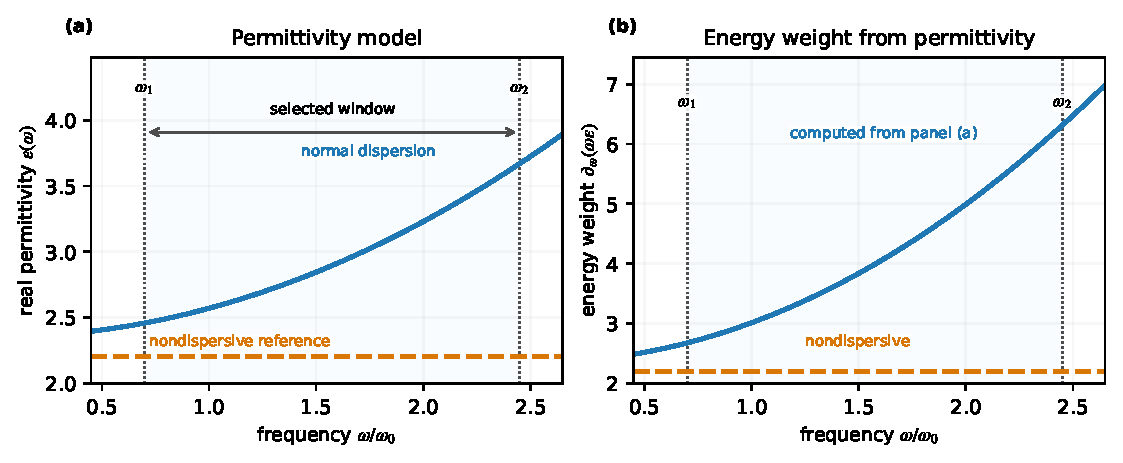
\includegraphics[width=0.92\textwidth]{figures/fig_ch03_dispersive_metric_step199.pdf}
  \caption{Dispersive energy metric and its frequency dependence.
  \textbf{(a)}~Representative dielectric function $\varepsilon(\omega)$
  of a Lorentzian medium, showing a selected lossless window between
  frequencies $\omega_1$ and $\omega_2$ where $\varepsilon$ is real and
  positive.  The dashed line marks the nondispersive reference level.
  \textbf{(b)}~The corresponding energy-metric weight
  $\partial_\omega[\omega\varepsilon(\omega)]$ computed from panel~(a).
  In the lossless window the weight exceeds unity and increases with
  frequency, reflecting the additional electromagnetic energy stored in
  the dispersive polarisation of the medium.  The orthogonality of
  Bloch modes in dispersive media
  (Theorem~\ref{thm:ch3-dispersive-orth}) is governed by this
  frequency-dependent metric rather than by $\varepsilon(\omega)$
  alone.}
  \label{fig:ch03-dispersive-metric}
\end{figure}


\begin{proof}
Start from the eigenvalue equations for modes $n$ and $m$:
\begin{align}
  \Maxop(\kvec)\,\mathbf{u}_n &= \omega_n\,\Mmat(\omega_n)\,\mathbf{u}_n\,,
  \label{eq:ch3-disp-evp-n}\\
  \Maxop(\kvec)\,\mathbf{u}_m &= \omega_m\,\Mmat(\omega_m)\,\mathbf{u}_m\,.
  \label{eq:ch3-disp-evp-m}
\end{align}
Take the inner product of \eqref{eq:ch3-disp-evp-m} with
$\mathbf{u}_n$ (standard $L^2$, with periodic boundary conditions as
before):
\begin{equation}
  \int\mathbf{u}_n^\dagger\,\Maxop(\kvec)\,\mathbf{u}_m\,\dd^3r
  = \omega_m\int\mathbf{u}_n^\dagger\,\Mmat(\omega_m)\,\mathbf{u}_m\,\dd^3r\,.
\end{equation}
By the self-adjointness of $\Maxop(\kvec)$ (the boundary term vanishes
for Bloch-periodic fields), the left-hand side also equals
$\int(\Maxop(\kvec)\mathbf{u}_n)^\dagger\mathbf{u}_m\,\dd^3r
=\omega_n^*\int\mathbf{u}_n^\dagger\Mmat^\dagger(\omega_n)\mathbf{u}_m\,\dd^3r
=\omega_n\int\mathbf{u}_n^\dagger\Mmat(\omega_n)\mathbf{u}_m\,\dd^3r$.
(We used $\omega_n\in\mathbb{R}$ and $\Mmat^\dagger=\Mmat$.)

Therefore:
\begin{equation}\label{eq:ch3-disp-orth-step}
  \omega_n\int\mathbf{u}_n^\dagger\Mmat(\omega_n)\mathbf{u}_m\,\dd^3r
  = \omega_m\int\mathbf{u}_n^\dagger\Mmat(\omega_m)\mathbf{u}_m\,\dd^3r\,.
\end{equation}
Equation~\eqref{eq:ch3-disp-orth-step} is already the desired exact
off-diagonal relation.  Equivalently,
\begin{equation}\label{eq:ch3-divided-difference-orth}
  \int \mathbf{u}_n^\dagger
  \left[
    \omega_n\Mmat(\omega_n)-\omega_m\Mmat(\omega_m)
  \right]
  \mathbf{u}_m\,\dd^3r = 0\,.
\end{equation}
For $n\neq m$ this may be viewed as orthogonality with respect to the
frequency divided-difference operator
\begin{equation}\label{eq:ch3-divided-difference-metric}
  \Mmat_{nm}^{\mathrm{dd}}
  = \frac{\omega_n\Mmat(\omega_n)-\omega_m\Mmat(\omega_m)}
  {\omega_n-\omega_m}\,.
\end{equation}
In the limit $\omega_m\to\omega_n$, this operator tends
$\partial_\omega[\omega\Mmat(\omega)]_{\omega_n}=\Mgmat(\omega_n)$.
Thus $\Mgmat$ is the correct self-overlap and near-degenerate metric,
while the exact off-diagonal relation for separated frequencies is the
divided-difference relation above.
\end{proof}

\begin{remark}
The proof shows that the energy metric $\Mgmat$ arises naturally as the
``linearisation'' of the nonlinear eigenvalue problem around a given
eigenfrequency.  The positive definiteness of $\Mgmat$ is not just a
convenient assumption; it is the physical stability condition ensuring
that each mode carries positive energy and that the eigenfrequencies
are locally non-degenerate as a function of $\omega$.
\end{remark}

\subsection{Normalisation in dispersive media}
\label{sec:ch3-disp-norm}

The natural normalisation convention for dispersive media is
\begin{equation}\label{eq:ch3-disp-norm}
  \boxed{%
  \eip{\mathbf{u}_n}{\mathbf{u}_m}
  \;\equiv\;
  \int_{\mathrm{cell}}
  \mathbf{u}_{n\kvec}^\dagger(\rvec)\,
  \Mgmat(\rvec,\omega_{n\kvec})\,
  \mathbf{u}_{m\kvec}(\rvec)\,\dd^3r
  = \delta_{nm}\,.}
\end{equation}
With this normalisation, the time-averaged electromagnetic energy stored
in the mode equals unity per unit cell, including the energy stored in
the material degrees of freedom (dispersive polarisation).

In the nondispersive limit $\partial\Mmat/\partial\omega=0$, the energy
metric reduces to $\Mgmat=\Mmat$ and
\eqref{eq:ch3-disp-norm} becomes \eqref{eq:ch3-normalisation}.

\subsection{Energy-weighted fields in dispersive media}
\label{sec:ch3-disp-weighted}

Since $\Mgmat(\omega)$ is Hermitian and positive definite at physical
eigenfrequencies, it also has a unique positive-definite square root.
Define
\begin{equation}\label{eq:ch3-disp-w}
  \emfieldw_{n\kvec}(\rvec)
  = \Mgmat^{1/2}(\rvec,\omega_{n\kvec})\,\mathbf{u}_{n\kvec}(\rvec)\,.
\end{equation}
Then $\int\emfieldw_n^\dagger\emfieldw_m\,\dd^3r=\delta_{nm}$, and all
Berry-geometry formulas can be written in terms of $\emfieldw$ with the
standard inner product.

\begin{remark}
There is a subtlety: $\Mgmat$ depends on $\omega_n(\kvec)$, which
varies with $\kvec$.  When computing Berry connections (derivatives
with respect to $\kvec$), one must account for this implicit $\kvec$
dependence through $\omega_n(\kvec)$.  We will address this carefully in
\chref{ch:geometry-bands}.
\end{remark}

\section{The role of the divergence constraint}
\label{sec:ch3-divergence}

The Maxwell curl equations \eqref{eq:ch3-evp-recap} are supplemented by
the divergence constraints $\nabla\cdot\Dfield=0$ and
$\nabla\cdot\Bfield=0$.  In the six-component formalism, these become
\begin{equation}\label{eq:ch3-div-constraint}
  \nabla\cdot\bigl(\Mmat\,\emfield\bigr) = 0\,,
\end{equation}
which in momentum space reads $(\kvec+\Gvec)\cdot(\Mmat\,\hat{\mathbf{u}}_\Gvec)=0$
for each Fourier component.

\paragraph{Transverse and longitudinal modes.}
For an isotropic medium with scalar $\varepsilon$ and $\mu$, the
eigenmodes of the Maxwell operator split into two classes:
\begin{itemize}
  \item \emph{Transverse modes} with $\kvec\cdot\Efield=0$ and
    $\kvec\cdot\Hfield=0$.  These have nonzero eigenfrequencies
    $\omega\neq0$ and represent propagating electromagnetic waves.
  \item \emph{Longitudinal modes} with $\nabla\times\Efield=0$ and
    $\nabla\times\Hfield=0$, satisfying
    $\Maxop\,\emfield_L=0$.  These are the null space of $\Maxop$
    and have $\omega=0$.
\end{itemize}
The divergence constraint eliminates the longitudinal modes from the
physical spectrum.  In a photonic crystal, the situation is analogous:
the physical modes lie in the transverse subspace satisfying
\eqref{eq:ch3-div-constraint}.

\begin{remark}
The longitudinal modes are often silently excluded in the photonic
band-structure literature by working directly with the second-order
equation $\nabla\times(\mu^{-1}\nabla\times\Efield)
=(\omega^2/c^2)\varepsilon\Efield$, which is automatically transverse
when applied to divergence-free fields.  The first-order six-component
formulation keeps them visible, which is important for rigour:
one must verify that the Berry curvature and Chern numbers are computed
only over the physical (transverse) bands.
\end{remark}

\section{Completeness and spectral theory}
\label{sec:ch3-completeness} \cite{initio2026pdf}

\subsection{Mode expansion}
\label{sec:ch3-expansion}

In a lossless nondispersive medium occupying a finite domain $V$ with
appropriate boundary conditions, the transverse eigenmodes
$\{\emfield_n\}$ of $\Hamop=\Mmat^{-1}\Maxop$ form a complete
orthonormal set with respect to the electromagnetic inner product.  Any
transverse six-component field can be expanded as
\begin{equation}\label{eq:ch3-mode-expansion}
  \emfield(\rvec) = \sum_n c_n\,\emfield_n(\rvec)\,,
  \qquad
  c_n = \emip{\emfield_n}{\emfield}\,.
\end{equation}
This is the electromagnetic analog of the expansion of a quantum state
in energy eigenstates.

For a periodic medium, completeness applies within each Bloch sector
at fixed $\kvec$: the cell-periodic modes
$\{\mathbf{u}_{n\kvec}\}_{n=1}^{\infty}$ span the transverse subspace
of $L^2$-periodic functions on the unit cell.

\subsection{Spectral properties}
\label{sec:ch3-spectral}

The eigenfrequencies $\omega_n(\kvec)$ are real and can be ordered:
\begin{equation}
  0 < \omega_1(\kvec) \leq \omega_2(\kvec) \leq \cdots\,.
\end{equation}
(We exclude the $\omega=0$ longitudinal modes.)  As $\kvec$ varies
over the Brillouin zone, each $\omega_n(\kvec)$ traces out a
\emph{band}.  The bands may overlap (when $\omega_n(\kvec)$ and
$\omega_{n+1}(\kvec')$ have the same value for different $\kvec,\kvec'$)
or may be separated by \emph{band gaps}: frequency intervals in which
no eigenfrequency exists for any $\kvec$.

The existence and width of band gaps depend on the contrast of the
material parameters and the geometry of the periodic structure.  We will
study the band structure in detail in \chref{ch:periodic-media}.

\section{Summary of key formulas}
\label{sec:ch3-summary}

For reference, we collect the central results of this chapter.

\begin{enumerate}
  \item \textbf{Electromagnetic inner product (nondispersive):}
  \begin{equation}
    \emip{\emfield_1}{\emfield_2}
    = \int_V\emfield_1^\dagger\,\Mmat\,\emfield_2\,\dd^3r\,.
    \tag{\ref{eq:ch3-em-ip}}
  \end{equation}

  \item \textbf{Self-adjointness:}
  $\Hamop=\Mmat^{-1}\Maxop$ is self-adjoint under $\langle\cdot,\cdot\rangle_\Mmat$.

  \item \textbf{Real eigenfrequencies, orthogonal modes:}
  $\omega_n\in\mathbb{R}$;\quad
  $\emip{\emfield_n}{\emfield_m}=\delta_{nm}$.

  \item \textbf{Energy-weighted field:}
  $\emfieldw=\Mmat^{1/2}\emfield$;\quad
  standard Hermitian eigenvalue problem for $\emfieldw$.

  \item \textbf{Dispersive energy metric:} \cite{gangaraj2016berry,silveirinha2016bulk}
  \begin{equation}
    \Mgmat(\omega)=\pderiv{}{\omega}[\omega\Mmat(\omega)]\,.
    \tag{\ref{eq:ch2-energy-metric}}
  \end{equation}

  \item \textbf{Orthogonality in dispersive media:}
  \begin{equation}
    \eip{\mathbf{u}_n}{\mathbf{u}_m}
    = \int_{\mathrm{cell}}
    \mathbf{u}_n^\dagger\,\Mgmat(\omega_n)\,\mathbf{u}_m\,\dd^3r
    = \delta_{nm}\,.
    \tag{\ref{eq:ch3-disp-norm}}
  \end{equation}
\end{enumerate}

These results are the foundation on which all Berry-geometric and
topological statements in the rest of the book are built.  The Berry
connection, Berry curvature, and Chern number for electromagnetic bands
must always be defined using the material-weighted inner product
$\langle\cdot,\cdot\rangle_\Mmat$ or its dispersive generalisation
$\langle\cdot,\cdot\rangle_{\Mgmat}$.  Using the wrong inner product---a
mistake easily made when importing formulas from quantum
mechanics---invalidates the topological invariants.

\section{The dispersive energy metric: derivation and meaning}
\label{sec:ch3-dispersive-derivation}

When the material parameters depend on frequency---as they must for
any causal material---the non-dispersive energy density
$\mathcal{U}=\frac{1}{2}\emfield^\dagger\Mmat(\omega)\emfield$ is
not the physically correct energy stored in the field.  The correct
expression is the Brillouin energy density, derived as follows.

\subsection{Derivation from energy conservation}
\label{sec:ch3-brillouin-derivation}

Consider a monochromatic field at frequency $\omega$ with a slowly
varying envelope.  The time-averaged energy density stored in the
medium is \cite{gangaraj2016berry}
\begin{equation}\label{eq:ch3-brillouin-energy}
  \langle\mathcal{U}\rangle
  = \frac{1}{4}\emfield^\dagger
  \frac{\partial[\omega\Mmat(\omega)]}{\partial\omega}\,\emfield
  = \frac{1}{4}\emfield^\dagger\Mgmat(\omega)\,\emfield\,.
\end{equation}
The dispersive energy metric $\Mgmat(\omega)
=\partial_\omega[\omega\Mmat(\omega)]$ appears because the energy
stored in the oscillators of the medium must be included alongside
the free-field energy.

For a non-dispersive material,
$\Mgmat=\Mmat+\omega\partial_\omega\Mmat=\Mmat$ (since
$\partial_\omega\Mmat=0$), and the Brillouin energy reduces to
the familiar non-dispersive form.

\subsection{Positivity from passivity}
\label{sec:ch3-positivity}

For a passive material (no gain), the Kramers--Kronig relations
guarantee that $\Mgmat(\omega)$ is positive definite at every
real frequency outside the absorption bands.  The physical argument
is simple: a passive material can only store (not create) energy,
so $\langle\mathcal{U}\rangle$ must be positive for all nonzero
field amplitudes \cite{silveirinha2016bulk}.

This positivity is essential for the entire topological framework of
this book: the electromagnetic inner product
$\eip{\emfield_1}{\emfield_2}
=\int\emfield_1^\dagger\Mgmat\,\emfield_2\,\dd^3 r$ is positive
definite, making the eigenproblem Hermitian and the Berry connection
well defined.  If $\Mgmat$ lost positive definiteness (as can happen
near a gain-induced instability), the Hermitian structure would break
and the Chern number would need to be redefined through the
non-Hermitian methods of Chapter~\ref{ch:non-hermitian}.

\subsection{The dispersive inner product and Berry connection}
\label{sec:ch3-dispersive-berry}

The dispersive energy metric enters the Berry connection through the
replacement $\Mmat\to\Mgmat$ everywhere the inner product appears.
Specifically, the Berry connection for band $n$ is
\begin{equation}\label{eq:ch3-dispersive-berry}
  \mathcal{A}_{n,a}(\kvec)
  = \ii\int_{\mathrm{cell}}
  \mathbf{u}_{n\kvec}^\dagger\,\Mgmat(\omega_{n\kvec})\,
  \partial_{k_a}\mathbf{u}_{n\kvec}\,\dd^3 r\,,
\end{equation}
where $\Mgmat(\omega_{n\kvec})$ is evaluated at the band frequency.
This formula reduces to the non-dispersive Berry connection when
$\Mgmat=\Mmat$, but it is the dispersive form that must be used for
real photonic crystals with frequency-dependent material response
\cite{gangaraj2016berry,ozawa2018topological}.

\section{Orthogonality subtleties}
\label{sec:ch3-orthogonality-subtleties}

\subsection{Degenerate modes and gauge freedom}
\label{sec:ch3-degenerate-gauge}

When two or more bands are degenerate at a point $\kvec_0$, the
individual modes $\mathbf{u}_{n\kvec_0}$ are not uniquely determined:
any unitary rotation within the degenerate subspace produces an
equally valid set of eigenmodes.  This gauge freedom means that the
Abelian Berry connection $\mathcal{A}_n$ is not well defined at
$\kvec_0$; instead, one must use the non-Abelian Berry connection
$\mathcal{A}_{mn}=\ii\eip{\mathbf{u}_m}{\nabla_\kvec\mathbf{u}_n}$,
where $m$ and $n$ range over the degenerate bands.

The non-Abelian connection transforms as a gauge field under unitary
rotations of the degenerate subspace, and its curvature
$\mathcal{F}_{mn}=\partial_a\mathcal{A}_{mn,b}
-\partial_b\mathcal{A}_{mn,a}
+\ii[\mathcal{A}_a,\mathcal{A}_b]_{mn}$
is gauge-covariant.  The Chern number of a degenerate band group is
$\Chern=\frac{1}{2\pi}\int_{\mathrm{BZ}}\Tr\,\mathcal{F}\,\dd^2 k$,
which is gauge-invariant and well defined even at the degeneracy
points \cite{gangaraj2016berry,ozawa2018topological}.

\subsection{Spurious modes and the null space}
\label{sec:ch3-spurious}

The Maxwell eigenproblem \eqref{eq:ch2-maxwell-matrix} admits spurious
static solutions ($\omega=0$) that satisfy
$\nabla\times\Efield=\nabla\times\Hfield=0$.  These are longitudinal
(gradient) fields that carry no energy and do not contribute to the
electromagnetic response.  In a photonic crystal calculation, they
appear as a flat band at $\omega=0$ and must be excluded from the
Berry-curvature computation.  The exclusion is automatic when one
restricts attention to bands at $\omega>0$, but numerical methods
must handle the near-zero modes carefully to avoid contamination of
the Chern-number calculation (Appendix~\ref{app:numerical-recipes})
\cite{price2022roadmap}.

\section{Worked example: modes of a uniform gyrotropic medium}
\label{sec:ch3-gyrotropic-example}

To illustrate the general theory concretely, we compute the normal
modes of a uniform gyrotropic medium with permittivity
$\varepsilon_r=15$ and Polder permeability
$\mu_\perp=3.47$, $\kappa_\mu=1.98$ (the YIG parameters of
Chapter~\ref{ch:microwave-crystal}).

For plane-wave solutions $\emfield\propto\ee^{\ii(\kvec\cdot\rvec-\omega t)}$
propagating along $\hat{z}$, the Maxwell eigenproblem reduces to
\begin{equation}\label{eq:ch3-gyrotropic-dispersion}
  k^2 = \frac{\omega^2}{c^2}\varepsilon_r\mu_\pm\,,
  \qquad
  \mu_\pm = \mu_\perp \mp \kappa_\mu\,,
\end{equation}
where $\mu_+=\mu_\perp-\kappa_\mu=1.49$ and
$\mu_-=\mu_\perp+\kappa_\mu=5.45$ are the eigenvalues of the
transverse permeability (Appendix~\ref{app:material-tensors}).
The two solutions correspond to right-circular (RCP, $+$) and
left-circular (LCP, $-$) polarisations with different phase
velocities $v_\pm=c/\sqrt{\varepsilon_r\mu_\pm}$.

The energy inner product for the RCP mode is
$\eip{\mathbf{u}_+}{\mathbf{u}_+}
=\frac{1}{4}(\varepsilon_0\varepsilon_r|E_+|^2+\mu_0\mu_+|H_+|^2)$,
which is positive definite since both $\varepsilon_r>0$ and
$\mu_+>0$ for the YIG parameters.  The RCP and LCP modes are
orthogonal under the energy inner product:
$\eip{\mathbf{u}_+}{\mathbf{u}_-}=0$, as guaranteed by
Theorem~\ref{thm:ch3-self-adjoint} \cite{gangaraj2016berry}.

The Faraday rotation angle per unit length is
$\theta_F=(k_+-k_-)/(2)
=(\omega/2c)\sqrt{\varepsilon_r}(\sqrt{\mu_+}-\sqrt{\mu_-})$,
providing a direct connection between the gyrotropic splitting and the
time-reversal-breaking perturbation that opens topological gaps in
photonic crystals.

\section{Completeness and expansion of arbitrary fields}
\label{sec:ch3-completeness-expansion}

\subsection{The completeness theorem}
\label{sec:ch3-completeness-theorem}

For a lossless, non-dispersive medium in a bounded domain $\Omega$
with appropriate boundary conditions, the normal modes
$\{\emfield_n\}_{n=1}^\infty$ form a complete orthonormal basis in the
Hilbert space $\mathcal{H}=L^2(\Omega;\Mmat\,\dd V)$.  Any
square-integrable field can be expanded as
\begin{equation}\label{eq:ch3-completeness-expansion}
  \emfield(\rvec) = \sum_n c_n\,\emfield_n(\rvec)\,,
  \qquad
  c_n = \eip{\emfield_n}{\emfield}\,,
\end{equation}
with convergence in the energy norm
$\|\emfield\|^2=\eip{\emfield}{\emfield}$.

The completeness is a consequence of the self-adjointness and the
compactness of the resolvent $(\Maxop-\omega\Mmat)^{-1}$ on the
bounded domain.  For an unbounded domain (such as a photonic crystal
with Bloch boundary conditions), the discrete sum is replaced by a
direct integral over the Brillouin zone
(Appendix~\ref{app:vector-identities})
\cite{silveirinha2016bulk,ozawa2018topological}.

\subsection{Subtleties of dispersive completeness}
\label{sec:ch3-dispersive-completeness}

For a dispersive medium, normal modes at different frequencies obey the
exact divided-difference orthogonality relation of
Theorem~\ref{thm:ch3-dispersive-orth}, rather than a simple
$\Mgmat(\omega_n)$ off-diagonal orthogonality rule.  The energy metric
$\Mgmat(\omega)$ appears in the self-overlap normalization and in the
near-degenerate limit, but modal expansions over a broad frequency range
must remember the frequency dependence of the material tensor.
However, the modes at a single fixed frequency do not form a complete
set for expanding fields at other frequencies, because the dispersive
energy metric $\Mgmat(\omega)$ is frequency-dependent.

This subtlety means that the modal expansion of a broadband pulse in a
dispersive medium requires modes at all frequencies, not just at a
single carrier frequency.  For topological photonics, this is usually
not a practical limitation because the operating bandwidth is much
narrower than the material dispersion range, and the modes can be
treated as non-dispersive within the topological gap
\cite{gangaraj2016berry,price2022roadmap}.

\section{Green's function formulation of topological invariants}
\label{sec:ch3-green-function}
\subsection{The gap Green's function}
\label{sec:ch3-gap-green}

For a frequency $\omega$ inside a band gap, the retarded Green's
function $G^R(\kvec;\omega)$ is analytic in $\kvec$ over the entire
Brillouin zone.  One first constructs the projector onto all bands
below the gap by a frequency-contour integral:
\begin{equation}\label{eq:ch3-green-projector}
  P(\kvec) = -\frac{1}{2\pi\ii}\oint_{\mathcal{C}}
  G^R(\kvec;\omega')\,\dd\omega'\,,
\end{equation}
where $\mathcal{C}$ is a contour in the complex frequency plane that
encloses all eigenfrequencies below the gap.
The gap Chern number is then the first Chern number of the image
bundle of $P(\kvec)$:
\begin{equation}\label{eq:ch3-green-chern}
  \Chern_{\mathrm{gap}}
  = \frac{1}{2\pi\ii}\int_{\mathrm{BZ}}\Tr\!\bigl[
    P\,\dd P\wedge\dd P
  \bigr]\,,
\end{equation}
where $\dd P=\partial_{k_x}P\,\dd k_x+\partial_{k_y}P\,\dd k_y$.
This formulation is gauge-invariant and naturally incorporates the
dispersive material response through the frequency-dependent Maxwell
operator inside $G^R$
\cite{web2026r,silveirinha2016bulk}.

\subsection{Advantages of the Green's function approach}
\label{sec:ch3-green-advantages}

The Green's function formulation has several advantages over the
eigenstate-based approach:

It avoids the gauge ambiguity inherent in choosing Bloch eigenstate
phases, because the Green's function is a gauge-invariant quantity.
It naturally includes the dispersive material response through the
frequency-dependent material tensor $\Mmat(\omega)$.  It extends
directly to non-Hermitian systems where the eigenstate Berry
connection is ill-defined due to the non-orthogonality of eigenmodes
\cite{web2026r,gao2015observation}.

The main computational disadvantage is that evaluating the Green's
function requires inverting the Maxwell operator at each $\kvec$
point, which is typically more expensive than a single eigenvalue
computation.  For practical band-structure calculations, the
eigenstate approach of Chapter~\ref{ch:computing-chern} remains
more efficient; the Green's function approach is most useful for
formal proofs of the bulk-edge correspondence and for systems where
the band structure is difficult to compute
\cite{silveirinha2016bulk,ozawa2018topological}.

\section{Mode completeness in practice}
\label{sec:ch3-completeness-practice}

The formal completeness of Maxwell normal modes becomes most useful
when it is translated into a field expansion.  Suppose first that the
medium is lossless, nondispersive, and enclosed in a volume with
boundary conditions that make the Maxwell generator self-adjoint in the
energy metric.  Let $\{\Psi_n\}$ be positive-frequency modes normalised
so that $\langle\Psi_m,\Psi_n\rangle_{\Mmat}=\delta_{mn}$.  A physical
field can then be expanded as
\begin{equation}\label{eq:ch3-modal-expansion}
  \Psi(\rvec,t)
  = \sum_{n>0}\left[a_n\Psi_n(\rvec)\ee^{-\ii\omega_n t}
  + a_n^*\mathcal{C}\Psi_n(\rvec)\ee^{+\ii\omega_n t}\right],
\end{equation}
where $\mathcal{C}$ denotes the particle-hole operation that maps a
positive-frequency Maxwell mode to its negative-frequency partner.  The
modal amplitude is obtained by projection,
\begin{equation}\label{eq:ch3-modal-amplitude}
  a_n = \langle\Psi_n,\Psi(0)\rangle_{\Mmat}.
\end{equation}
This formula is the electromagnetic analogue of expanding a quantum
state in energy eigenstates, but the projection uses stored energy.
Using a flat $L^2$ projection would give wrong amplitudes whenever the
field energy is distributed unevenly between electric and magnetic
components or between field and material oscillators.

In a periodic medium the same statement holds fibre by fibre in Bloch
momentum.  A finite-energy wave packet centred near a band $n$ and wave
vector $\kvec_0$ has the form
\begin{equation}\label{eq:ch3-bloch-wavepacket}
  \Psi(\rvec,t)
  =\int_{\mathrm{BZ}} A_n(\kvec)
  \ee^{\ii\kvec\cdot\rvec-\ii\omega_n(\kvec)t}
  u_{n\kvec}(\rvec)\,\frac{\dd^d k}{(2\pi)^d}+	ext{c.c.},
\end{equation}
with $u_{n\kvec}$ normalised in the unit-cell energy metric.  The
slow variation of the eigenmode $u_{n\kvec}$ across the packet in
$\kvec$-space is precisely what produces Berry connection and Berry
curvature in Chapter~\ref{ch:geometry-bands}.  Thus Berry geometry is
not an optional decoration added after solving the Maxwell eigenproblem;
it is already present in the way neighbouring normal modes are compared.

\section{Green functions as spectral projectors}
\label{sec:ch3-green-projector-practice}

The modal expansion also explains why Green functions appear naturally
in topological photonics
\cite{hsu2016bound}.  For a nondispersive lossless system, the
resolvent of the Maxwell generator is
\begin{equation}\label{eq:ch3-resolvent-modal}
  G(z)=(z-\hat{H}_{\mathrm{M}})^{-1}
  =\sum_n \frac{|\Psi_n\rangle\langle\Psi_n|_{\Mmat}}{z-\omega_n},
\end{equation}
where $\langle\Psi_n|_{\Mmat}$ means the dual vector defined by the
energy inner product.  If a closed contour $\Gamma$ in the complex
$z$-plane surrounds a group of bands and no other spectrum, the
spectral projector is
\begin{equation}\label{eq:ch3-contour-projector-expanded}
  P_\Gamma = \frac{1}{2\pi\ii}\oint_\Gamma G(z)\,\dd z.
\end{equation}
This projector is independent of the basis chosen inside the band
subspace.  It is therefore the natural object for non-Abelian Berry
curvature, Wilson loops, and numerical Chern calculations in nearly
degenerate photonic bands \cite{silveirinha2016bulk,unknown2008a}.

For dispersive media the same idea survives, but the residues of the
Green function are weighted by the Brillouin energy metric.  This is why
Green-function formulas for photonic Chern numbers must be handled with
care: poles in frequency are not simply poles of a Hermitian matrix
with a constant metric.  The mathematically safe procedure is either to
embed the dispersive material into an enlarged auxiliary-field
Hamiltonian or to use the divided-difference orthogonality relations
introduced earlier in this chapter.  Both routes preserve the same
physical statement: topology belongs to the spectral projector onto a
bundle of Maxwell modes, not to an arbitrary choice of mode basis.

\begin{figure}[t]
  \centering
  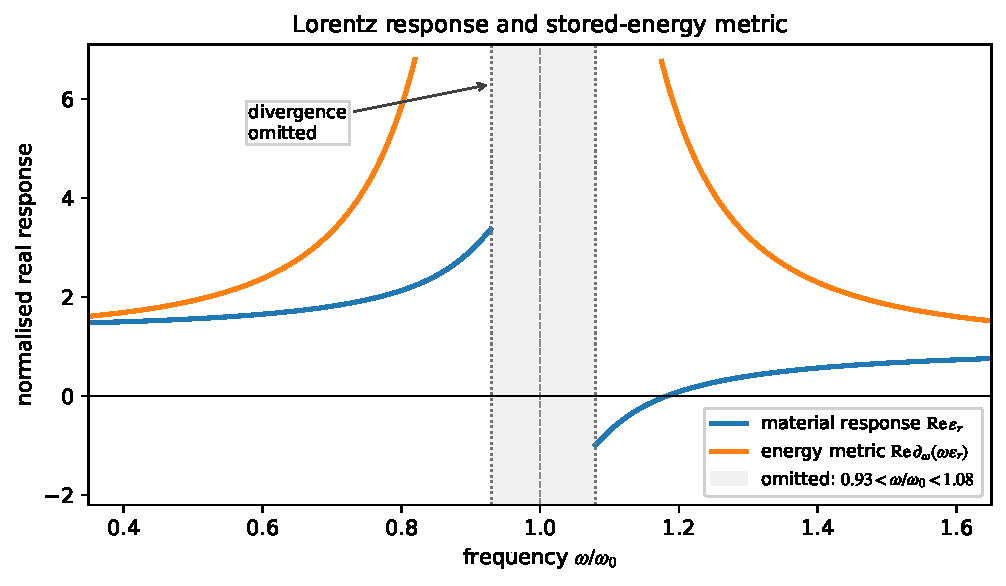
\includegraphics[width=0.82\textwidth]{figures/fig_ch03_energy_metric.pdf}
  \caption{A dispersive material illustrates why the electromagnetic
  inner product uses the energy derivative $\partial_\omega[\omega\varepsilon]$
  rather than the static permittivity alone.  Near a material resonance,
  the static response and the positive-energy metric can differ strongly.}
  \label{fig:ch03-energy-metric}
\end{figure}

\section*{Exercises}

\begin{exercise}
  For a uniform medium with $\Mmat=\diag(\varepsilon_0\varepsilon,
  \varepsilon_0\varepsilon,\varepsilon_0\varepsilon,
  \mu_0\mu,\mu_0\mu,\mu_0\mu)$, compute $\Mmat^{1/2}$ explicitly and
  verify that the energy-weighted operator
  $\tilde{\Hamop}=\Mmat^{-1/2}\Maxop(\kvec)\Mmat^{-1/2}$ is Hermitian
  by direct matrix computation for $\kvec=k\hat{z}$.
\end{exercise}

\begin{exercise}
  Consider a Drude plasma with $\varepsilon(\omega)=1-\omega_p^2/\omega^2$
  and $\mu=1$.  Compute the energy metric $\Mgmat(\omega)$ and verify
  that it is positive definite for $\omega>\omega_p$.  What happens at
  $\omega=\omega_p$?  Interpret physically.
\end{exercise}

\begin{exercise}
  For the gyrotropic permeability \eqref{eq:ch2-gyrotropic-mu}, suppose
  that $\mu_\perp(\omega)$, $\kappa(\omega)$, and $\mu_z(\omega)$ are
  given by the Polder model for a magnetised ferrite:
  \begin{equation}
    \mu_\perp = 1 + \frac{\omega_0\omega_m}{\omega_0^2-\omega^2}\,,
    \qquad
    \kappa = \frac{\omega\omega_m}{\omega_0^2-\omega^2}\,,
    \qquad
    \mu_z = 1\,,
  \end{equation}
  where $\omega_0$ is the Larmor frequency and $\omega_m$ is the
  saturation-magnetisation frequency.  Compute the $\mut$-block of
  $\Mgmat(\omega)$ and determine the frequency range over which it is
  positive definite.
\end{exercise}

\begin{exercise}
  Prove that in a periodic medium with Bloch boundary conditions, the
  surface integral in \eqref{eq:ch3-boundary-term} vanishes.
  \emph{Hint:} pair opposite faces of the unit cell and use the
  Bloch phase relation
  $\emfield(\rvec+\avec)=\ee^{\ii\kvec\cdot\avec}\emfield(\rvec)$.
\end{exercise}

\begin{exercise}[Longitudinal modes]
  Show that in a homogeneous isotropic medium, the six-component fields
  $\emfield_L=(\nabla\phi,\mathbf{0})^T$ (for arbitrary scalar $\phi$)
  and $\emfield_L'=(\mathbf{0},\nabla\psi)^T$ satisfy
  $\Maxop\emfield_L=0$ and $\Maxop\emfield_L'=0$.  Verify that they
  are orthogonal to every transverse mode under $\langle\cdot,\cdot\rangle_\Mmat$.
\end{exercise}

\begin{exercise}
  The dispersive inner product $\langle\cdot,\cdot\rangle_{\Mgmat}$
  involves $\Mgmat(\omega_n)$ evaluated at the eigenfrequency of mode~$n$.
  Show that for two degenerate modes at the same frequency
  ($\omega_n=\omega_m$), the inner product is well defined and reduces to
  the ordinary Hermitian form $\int\mathbf{u}_n^\dagger\Mgmat\mathbf{u}_m\,\dd^3r$.
\end{exercise}
